\section{Supły} % (fold)
\label{sec:tangle}

Na przełomie lat sześćdziesiątych i~siedemdziesiątych Conway szukał sposobu na zbudowanie kompletnej tablicy węzłów.
Niezmienniki znane w~tym czasie nie były dostatecznie mocne, by sprostać temu wyzwaniu.
Conway wprowadził pojęcie supła i~chociaż wszystkich węzłów nie można z~nich uzyskać, teoria została pchnięta do przodu.
Supły stanowią budulec splotów takich jak na przykład precle z~definicji \ref{def:pretzel}.

Sekcja oparta jest na podręczniku Murasugiego \cite{murasugi96} i~pracach \cite{conway70}, \cite{kauffman97}, \cite{kauffman04}, a~także \cite{schubert56}.
Po raz pierwszy z~supłami zetknęliśmy się w~pracy \cite{janiak04}, także czerpiącej inspirację z~\cite{murasugi96}, choć podejrzewamy, że konwencje nazewnicze w tych pracach wzajemnie wykluczają się.

\begin{definition}[supeł]
    \label{def:tangle}
    \index{supeł}
    Zawarty w~kole fragment diagramu splotu o~dwóch łukach wyjściowych oraz dwóch wejściowych, nazywamy supłem.
\end{definition}

Istnieją dwa rodzaje supłów -- naprzemienne i~sąsiadujące.
\begin{center}
	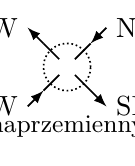
\begin{tikzpicture}[baseline=-0.65ex, scale=0.1]
	\useasboundingbox (-5, -9) rectangle (5, 5);
		\node [left] at (-5, -5) {SW};
		\draw[semithick,latex-] (-3, -3) to (-5,-5);
		\draw[semithick] (-3, -3) to (-1,-1);
		\node [right] at (5, 5) {NE};
		\draw[semithick,latex-] (3, 3) to (5,5);
		\draw[semithick] (3, 3) to (1,1);
		\node [right] at (5, -5) {SE};
		\draw[semithick,-latex] (3, -3) to (5,-5);
		\draw[semithick] (3, -3) to (1,-1);
		\node [left] at (-5, 5) {NW};
		\draw[semithick,-latex] (-3, 3) to (-5,5);
		\draw[semithick] (-3, 3) to (-1,1);
		\draw[semithick, densely dotted] (-0, 0) circle (3);
		\node at (0, -5) [below] {\small naprzemienny};
	\end{tikzpicture}
	\quad\quad\quad\quad\quad\quad
	\begin{tikzpicture}[baseline=-0.65ex, scale=0.1]
	\useasboundingbox (-5, -9) rectangle (5, 5);
		\node [left] at (-5, -5) {SW};
		\draw[semithick,latex-] (-3, -3) to (-5,-5);
		\draw[semithick] (-3, -3) to (-1,-1);
		\node [right] at (5, 5) {NE};
		\draw[semithick,-latex] (3, 3) to (5,5);
		\draw[semithick] (3, 3) to (1,1);
		\node [right] at (5, -5) {SE};
		\draw[semithick,latex-] (3, -3) to (5,-5);
		\draw[semithick] (3, -3) to (1,-1);
		\node [left] at (-5, 5) {NW};
		\draw[semithick,-latex] (-3, 3) to (-5,5);
		\draw[semithick] (-3, 3) to (-1,1);
		\draw[semithick, densely dotted] (-0, 0) circle (3);
		\node at (0, -5) [below] {\small sąsiadujący};
	\end{tikzpicture}
\end{center}

Podobnie jak dla węzłów, pojawia się naturalne pytanie o~równoważność dwóch supłów.
Jest tak wtedy, gdy istnieje homeomorfizm* kuli na siebie, który przekształca jeden supeł na drugi, ale nie rusza sfery otaczającej.
Dla diagramów odpowiada to ruchom Reidemeistera, nie mamy jednak prawa opuszczać kuli zawierającej supeł.

Wszystkich supłów jest bardzo dużo, więc ograniczymy się do końca rozdziału do pewnej ich regularnej rodziny.
Oto cztery podstawowe supły:
\[
    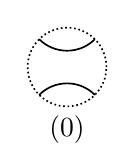
\begin{tikzpicture}[baseline=-0.65ex, scale=0.1]
    \useasboundingbox (-5, -9) rectangle (5, 5);
        \draw[semithick] (-5 / 1.4142, -5 / 1.4142) [in=135, out=45] to (5 / 1.4142, -5 / 1.4142);
        \draw[semithick] (-5 / 1.4142, 5 / 1.4142) [in=-135, out=-45] to (5 / 1.4142, 5 / 1.4142);
        \draw[semithick, densely dotted] (-0, 0) circle (5);
        \node at (0, -5) [below] {$(0)$};
    \end{tikzpicture}
    \quad\quad\quad
    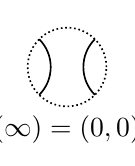
\begin{tikzpicture}[baseline=-0.65ex, scale=0.1]
    \useasboundingbox (-5, -9) rectangle (5, 5);
        \draw[semithick] (-5 / 1.4142, -5 / 1.4142) [in=-45, out=45] to (-5 / 1.4142, 5 / 1.4142);
        \draw[semithick] (5 / 1.4142, -5 / 1.4142) [in=-135, out=135]  to (5 / 1.4142, 5 / 1.4142);
        \draw[semithick, densely dotted] (-0, 0) circle (5);
        \node at (0, -5) [below] {$(\infty) = (0, 0)$};
    \end{tikzpicture}
    \quad\quad\quad
    \begin{tikzpicture}[baseline=-0.65ex, scale=0.1]
    \useasboundingbox (-5, -9) rectangle (5, 5);
    \begin{knot}[clip width=5, end tolerance=1pt]
        \strand[semithick] (-5 / 1.4142, -5 / 1.4142) to (5 / 1.4142, 5 / 1.4142);
        \strand[semithick] (5 / 1.4142, -5 / 1.4142) to (-5 / 1.4142, 5 / 1.4142);
        \strand[semithick, densely dotted] (-0, 0) circle (5);
        \node at (0, -5) [below] {$(-1)$};
    \end{knot}
    \end{tikzpicture}
    \quad\quad\quad
    \begin{tikzpicture}[baseline=-0.65ex, scale=0.1]
    \useasboundingbox (-5, -9) rectangle (5, 5);
    \begin{knot}[clip width=5, end tolerance=1pt, flip crossing/.list={1}]
        \strand[semithick] (-5 / 1.4142, -5 / 1.4142) to (5 / 1.4142, 5 / 1.4142);
        \strand[semithick] (-5 / 1.4142, 5 / 1.4142) to (5 / 1.4142, -5 / 1.4142);
        \strand[semithick, densely dotted] (-0, 0) circle (5);
        \node at (0, -5) [below] {$(1)$};
    \end{knot}
    \end{tikzpicture}
\]

\begin{definition}
    \label{def:rational_tangle}
    Supły powstające z~$(0)$ lub $(\infty)$ przez homeomorfizm kuli na siebie permutujący wejścia i~wyjścia nazywamy wymiernymi.
\end{definition}

Wystarczy się przy tym ograniczyć do ciągu obrotów półsfery dolnej (SW--SE) oraz lewej (SW--NW)
Z obrotami prawoskrętnymi wiążemy liczby dodatnie, natomiast z~lewoskrętnymi -- ujemne.
Otrzymujemy tak pewną krotkę $(a_1, \ldots, a_n)$.
Jeśli $n$ jest parzyste, zaczynamy od supła $(\infty)$, jeśli nie -- od $(0)$.
Ostatni obrót dotyczy półsfery dolnej.
Krotka nie jest jeszcze niezmiennikiem supłów (gdyż $(-2,3,3) \cong (3, -2, 3)$), ale nic straconego.
Potrzebować będziemy prostej definicji, uzasadniającej określenie ,,supły wymierne''.
% Conway pokazał, że dla dowolnego supła przy pomocy wielomianu Alexandera zdefiniować można  pewien ułamek.

\begin{proposition}
\label{prp:continued_fractions}
    Istnieje bijekcja między klasami supłów wymiernych oraz łańcuchowymi ułamkami, które je przedstawiają:
    \[
        \frac \alpha \beta = a_n + \frac{1}{a_{n-1} + 1 / (a_{n-2} +  \ldots + 1/a_1)} \in \Q \cup \{\infty\}.
    \]
\end{proposition}

\begin{proof}
    Praca \cite{conway70} Conwaya.
\end{proof}

\begin{proposition}
\label{prp:continued_fractions_2}
    Supły o~łańcuchowych ułamkach różnych od $0$ i~$\infty$ można kodować ciągami liczb całkowitych tego samego znaku.
\end{proposition}

Z każdym supłem $T$ związane jest jego odbicie $\overline T$, obraz wyjściowego przez symetrię względem prostej $y = -x$.
Mając dwa supły obok siebie, można dokonać ich sklejenia wzdłuż połówek kul, w~których leżą:
\[
    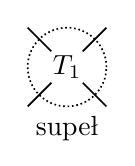
\begin{tikzpicture}[baseline=-0.65ex, scale=0.1]
    \useasboundingbox (-5, -9) rectangle (5, 5);
        \draw[semithick] (-2, -2) to (-5,-5);
        \draw[semithick] (2, 2) to (5,5);
        \draw[semithick] (2, -2) to (5,-5);
        \draw[semithick] (-2, 2) to (-5,5);        %
        \draw[semithick, densely dotted] (-0, 0) circle (5);
        \node at (0, 0) {$T_1$};
        \node [below] at (0, -5) {supeł};
    \end{tikzpicture}
    \quad \quad
    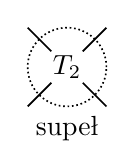
\begin{tikzpicture}[baseline=-0.65ex, scale=0.1]
    \useasboundingbox (-5, -9) rectangle (5, 5);
        \draw[semithick] (-2, -2) to (-5,-5);
        \draw[semithick] (2, 2) to (5,5);
        \draw[semithick] (2, -2) to (5,-5);
        \draw[semithick] (-2, 2) to (-5,5);        %
        \draw[semithick, densely dotted] (-0, 0) circle (5);
        \node at (0, 0) {$T_2$};
        \node [below] at (0, -5) {supeł};
    \end{tikzpicture}
    \quad \quad
    % \begin{tikzpicture}[baseline=-0.65ex, scale=0.1]
    % \useasboundingbox (-15, -9) rectangle (15, 5);
    %     \draw[semithick] (-12, -2) to (-15,-5);
    %     \draw[semithick] (-12, 2) to (-15,5);        %
    %     \draw[semithick, densely dotted] (-10, 0) circle (5);
    %     \node at (-10, 0) {$T_1$};
    %     \draw[semithick] (12, -2) to (15,-5);
    %     \draw[semithick] (12, 2) to (15,5);        %
    %     \draw[semithick, densely dotted] (10, 0) circle (5);
    %     \node at (10, 0) {$T_2$};
    %     \draw[semithick] (-8, 2) [in=135, out=45] to (8, 2);
    %     \draw[semithick] (-8, -2) [in=-135, out=-45] to (8, -2);
    %     \node [below] at (0, -5) {produkt};
    % \end{tikzpicture}
    % \quad \quad
    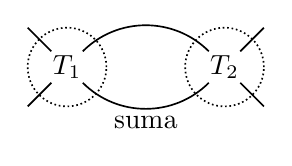
\begin{tikzpicture}[baseline=-0.65ex, scale=0.1]
    \useasboundingbox (-15, -9) rectangle (15, 5);
        \draw[semithick] (-12, -2) to (-15,-5);
        \draw[semithick] (-12, 2) to (-15,5);        %
        \draw[semithick, densely dotted] (-10, 0) circle (5);
        \node at (-10, 0) {$T_1$};
        \draw[semithick] (12, -2) to (15,-5);
        \draw[semithick] (12, 2) to (15,5);        %
        \draw[semithick, densely dotted] (10, 0) circle (5);
        \node at (10, 0) {$T_2$};
        \draw[semithick] (-8, 2) [in=135, out=45] to (8, 2);
        \draw[semithick] (-8, -2) [in=-135, out=-45] to (8, -2);
        \node [below] at (0, -5) {suma};
    \end{tikzpicture}
\]

Oznaczmy tak otrzymany węzeł przez $T_1 + T_2$.
Niektórzy definiują dalsze działania, jak produkt: $T_1 \cdot T_2 = \overline T_1 + T_2$ czy rozgałęzienie, $\overline T_1 + \overline T_2$.
Rodzina supłów wymiernych jest zamknięta na branie produktów, ale nie sum.
Wprowadzamy więc następującą, ogólniejszą definicję.
Supeł będący skończoną sumą supłów wymiernych, ich luster, odbić lub odbić luster nazywamy algebraicznym.

Przez zszycie par łuków wejściowych (lub wyjściowych) zamieniamy supły w~węzły:
\begin{comment}
\[
    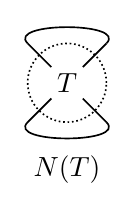
\begin{tikzpicture}[baseline=-0.65ex, scale=0.1]
    \useasboundingbox (-5, -11) rectangle (5, 7);
        \draw[semithick] (-2, -2) to (-5,-5);
        \draw[semithick] (2, 2) to (5,5);
        \draw[semithick] (2, -2) to (5,-5);
        \draw[semithick] (-2, 2) to (-5,5);        %
        \draw[semithick, densely dotted] (-0, 0) circle (5);
        \node at (0, 0) {$T$};
        \node [below] at (0, -8) {$N(T)$};
        \draw[semithick] (-5, -5) [in=-45, out=-135] to (5, -5);        %
        \draw[semithick] (-5,    5) [in=45, out=135] to (5, 5);        %
    \end{tikzpicture}
    \quad \quad
    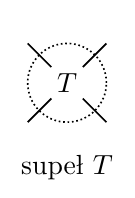
\begin{tikzpicture}[baseline=-0.65ex, scale=0.1]
    \useasboundingbox (-5, -11) rectangle (5, 7);
        \draw[semithick] (-2, -2) to (-5,-5);
        \draw[semithick] (2, 2) to (5,5);
        \draw[semithick] (2, -2) to (5,-5);
        \draw[semithick] (-2, 2) to (-5,5);        %
        \draw[semithick, densely dotted] (-0, 0) circle (5);
        \node at (0, 0) {$T$};
        \node [below] at (0, -8) {supeł $T$};
    \end{tikzpicture}
    \quad \quad
    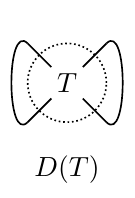
\begin{tikzpicture}[baseline=-0.65ex, scale=0.1]
    \useasboundingbox (-5, -11) rectangle (5, 7);
        \draw[semithick] (-2, -2) to (-5,-5);
        \draw[semithick] (2, 2) to (5,5);
        \draw[semithick] (2, -2) to (5,-5);
        \draw[semithick] (-2, 2) to (-5,5);        %
        \draw[semithick, densely dotted] (-0, 0) circle (5);
        \node at (0, 0) {$T$};
        \node [below] at (0, -8) {$D(T)$};
        \draw[semithick] (-5, -5) [in=135, out=-135] to (-5, 5);        %
        \draw[semithick] (5, -5) [in=45, out=-45] to (5, 5);        %
    \end{tikzpicture}
    \quad \quad
\]
\end{comment}

Oznaczenia $N(T)$ oraz $D(T)$ pochodzą od angielskich słów \emph{numerator}, \emph{denominator}.
Być może nie jest jasne, dlaczego terminy stosowane zazwyczaj do opisu ułamków stosujemy wobec diagramów splotów.
Nazewnictwo nie jest przypadkowe. %, wrócimy do tego tematu wkrótce.
\begin{proposition}
\label{prp:knot_fraction}
    Ułamek supła zadany wzorem
    \[
        F(A) = \frac{\nabla_{N(A)}(z)}{\nabla_{D(A)}(z)}
    \]
    spełnia zależność $F(A+B) = F(A) + F(B)$.
\end{proposition}

\begin{proof}
    Praca \cite{conway70} Conwaya.
\end{proof}

Istnieją supły $T_1$, $T_2$ takie, że węzły $N(T_i)$ są nietrywialne, ale $N(T_1 + T_2)$ to niewęzeł.
Co gorsza, dla każdego wymiernego supła $A$ istnieje taki supeł $B$, że $N(A+B)$ jest niewęzłem.

Praca \cite{conway70} zawiera jeszcze jeden ciekawy rezultat, uogólniony przez Lickorisha i~Milletta w~\cite{lickorish87}.
Przyjmijmy następujące skróty: niech $A_n = P_{N(A)}(x,y)$, $A_d = P_{D(A)}(x,y)$.

\begin{proposition}
    Dla dowolnych supłów $A, B$ mamy
    \[
    (1 - (x+y)^2)(A+B)_n = (A_nB_d + A_dB_n) - (x+y)(A_nB_n+  A_dB_d)
    \]
    oraz
    \[
        (A+B)_d = A_dB_d.
    \]
\end{proposition}

Uwaga, zastosowano tu nieco inną parametryzację wielomianu HOMFLY.
Na zakończenie wspomnimy o~mutacjach.

\begin{definition}[mutacja]
\label{def:mutant}
    Półobrót supła względem osi poziomej, pionowej albo też prostopadłej do płaszczyzny, w~jakiej leży diagram, nazywamy mutacją, zaś otrzymany tak splot -- mutantem.
    W razie potrzeby zmieniamy orientację supła na przeciwną.
\end{definition}

Mutacja węzła o~co najwyżej dziesięciu skrzyżowaniach nie zmienia jego klasy abstrakcji.
Najsłynniejszą parę mutantów stanowią węzeł Conwaya oraz Kinoshity-Terasakiego.
Dowód ich nierównoważności podał jako pierwszy prawdopodobnie Riley w~1971 \cite{riley71}:
wykorzystał on homomorfizmy z~grupy węzła w~$PSL(2, 7)$.
Genusy (odpowiednio: $3$ i~$2$) wyznaczył Gabai w~1986 roku \cite{gabai86}, używał foliacji.

Livingston pokazał istnienie mutantów o~różnym genusie plastrowym.
% TODO: C Livingston, Knots which are not concordant to their reverses, Quart. J. Math. Oxford (Ser. 2) 34 (1983) 323–328
Nie wiadomo, czy mutacja jest w~stanie zmienić liczbę gordyjską.
Gordon i~Luecke pokazali w~2006, że rodzina węzłów $1$-gordyjskich jest zamknięta na mutacje (\cite{gordon06}).
Dużo wcześniej wiedzieliśmy tylko, że jedynym mutantem niewęzła jest niewęzeł (Rolfsen w~\cite{rolfsen93}?).
Mutacja nie zmienia sygnatury.
Mutacja alternującego diagramu jest alternującym węzłem.

Chmutov, Duzhin oraz Lando pokazali, że niezmienniki Wasiljewa stopnia co najwyżej ósmego nie rozróżniają mutantów (\cite{chmutov94} z~1994).
Wynik poprawił Murakami do dziesiątego stopnia (,,Finite type invariants detecting the mutant knots'' z~2000 roku, dostępny na stronie internetowej autora) i~potwierdził, że pewien niezmiennik stopnia 11 (używany przez Mortona i~Cromwella) odróżnia węzeł Conwaya od węzła Kinoshity-Terasakiego.

Niedawno Stojmenow podjął się systematycznie znalezienia mutantów wśród węzłów o~mniej niż dziewiętnastu skrzyżowaniach (praca \cite{stoimenow10} z~2010 roku).

\subsection{Sploty o~dwóch mostach} % (fold)
\label{sub:twobridge}
Zajmiemy się teraz związkiem supłów z indeksem mostowym.
Wiemy, że węzeł trywialny jest jednomostowy, następne w hierarchii są sploty dwumostowe.
Nazywa się je także wymiernymi, po angielsku czasami \emph{4-plats}.
Jako pierwszy studiował je Bankwitz z~Schumannem w~1934 roku.
% Kawauchi: as 4-plat presentations, which is just Conway's normal form.
Mają co najwyżej dwie składowe i~są odwracalne.

\begin{proposition}
    Sploty dwumostowe są pierwsze.
\end{proposition}

\begin{proof}
    Prosty wniosek z~tego, że liczba mostowa prawie jest addytywna (fakt \ref{prp:bridge_additive}).
\end{proof}

\begin{corollary}
    Węzły dwumostowe są $(\pm 2, n)$-torusowe albo hiperboliczne.
\end{corollary}

\begin{tobedone}
    % Skorzystajmy z trychotomii Thurstona: węzły dwumostowe są pierwsze, zatem nie są satelitarne.
    % Pozostało rozpatrzyć przypadek, kiedy nie są hiperboliczne.
    Teza wynika wtedy bezpośrednio z faktu \ref{prp:torus_bridge_number}, który głosi, że $br(T_{p, q}) = \min\{|p|, |q|\}$.
\end{tobedone}

\begin{proposition}
    Pierwsze węzły trzymostowe są $(\pm 3, n)$-torusowe albo hiperboliczne.
\end{proposition}

\begin{proof}
    Wniosek 10.5.2 w \cite{kawauchi96}, ale z innego twierdzenia.
\end{proof}

%\todo[inline]{Murasugi Theorem 9.3.3 (138) lub Janiak-Osajca, Pogoda (34).}
% Aus der unten stehenden Klassifikation ergibt sich, dass man jede Verschlingung mit 2 Brücken wie im Bild rechts darstellen kann, wobei {\displaystyle a_{i}\in \mathbb {Z} } a_{i}\in \mathbb{Z }  die Anzahl der Halbtwists in der jeweiligen Box bezeichnet und für gerade bzw. ungerade {\displaystyle i} i~positive {\displaystyle a_{i}} a_{i} links- bzw. rechtshändigen Halbtwists entsprechen.
% Diese Darstellung wird als Conway-Normalform bezeichnet.
% Man kann stets erreichen, dass alle {\displaystyle a_{i}} a_{i} dasselbe Vorzeichen haben.[1] Insbesondere gibt die Conway-Normalform dann ein alternierendes Knotendiagramm.[2]
%Insbesondere ist ein 2-Brücken-Knoten genau dann amphichiral, wenn {\displaystyle q^{2}\equiv -1\ mod\ p} q^{2}\equiv -1\ mod\ p ist.

\begin{proposition}
    Sploty z~dwoma mostami to dokładnie sploty typu $D(T)$ dla pewnego supła wymiernego $T$.
\end{proposition}

Dowód tego stwierdzenia znaleźć można na przykład w książce \cite{murasugi96}, strony 183-187.
Wynika z niego, że każdy splot dwumostowy można przedstawić następującym diagramem:
\[
	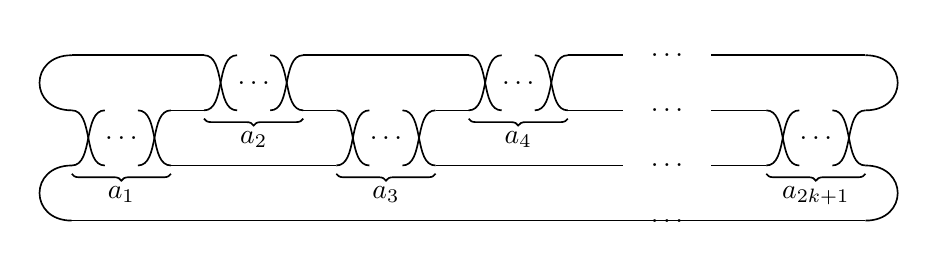
\begin{tikzpicture}[baseline=-0.65ex, xscale=0.14, yscale=0.07]
	\useasboundingbox (-40, -20) rectangle (40, 20);
		%%% A1
		\draw[semithick] (-36, -5) .. controls (-34,-5) and (-35, 5) .. (-33, 5);
		\draw[semithick] (-36,  5) .. controls (-34, 5) and (-35,-5) .. (-33,-5);
		\node at (-31.5, 0) {$\ldots$};
		\draw[semithick] (-30, -5) .. controls (-28,-5) and (-29, 5) .. (-27, 5);
		\draw[semithick] (-30,  5) .. controls (-28, 5) and (-29,-5) .. (-27,-5);
		%%% A2
		\draw[semithick] (-24,  5) .. controls (-22,  5) and (-23, 15) .. (-21, 15);
		\draw[semithick] (-24, 15) .. controls (-22, 15) and (-23,  5) .. (-21,  5);
		\node at (-19.5, 10) {$\ldots$};
		\draw[semithick] (-18,   5) .. controls (-16,  5) and (-17, 15) .. (-15, 15);
		\draw[semithick] (-18,  15) .. controls (-16, 15) and (-17,  5) .. (-15,  5);
		%%% A3
		\draw[semithick] (-12, -5) .. controls (-10,-5) and (-11, 5) .. (-9, 5);
		\draw[semithick] (-12,  5) .. controls (-10, 5) and (-11,-5) .. (-9,-5);
		\node at (-7.5, 0) {$\ldots$};
		\draw[semithick] (-6, -5) .. controls (-4,-5) and (-5, 5) .. (-3, 5);
		\draw[semithick] (-6,  5) .. controls (-4, 5) and (-5,-5) .. (-3,-5);
		%%% A4
		\draw[semithick] (0,  5) .. controls (2,  5) and (1, 15) .. (3, 15);
		\draw[semithick] (0, 15) .. controls (2, 15) and (1,  5) .. (3,  5);
		\node at (4.5, 10) {$\ldots$};
		\draw[semithick] (6,   5) .. controls (8,  5) and (7, 15) .. (9, 15);
		\draw[semithick] (6,  15) .. controls (8, 15) and (7,  5) .. (9,  5);
		%%% A 2k+1
		\draw[semithick] (27,  -5) .. controls (29,  -5) and (28, 5) .. (30, 5);
		\draw[semithick] (27, 5) .. controls (29, 5) and (28,  -5) .. (30,  -5);
		\node at (31.5, 0) {$\ldots$};
		\draw[semithick] (33,   -5) .. controls (35,  -5) and (34, 5) .. (36, 5);
		\draw[semithick] (33,  5) .. controls (35, 5) and (34,  -5) .. (36,  -5);
		%%%    - A3
		\draw[semithick] (-36, 15) to (-24, 15);
		%%% A1 - A3
		\draw[semithick] (-27, -5) to (-12, -5);
		%%% A1 - A2
		\draw[semithick] (-27,  5) to (-24,  5);
		%%% A2 - A3
		\draw[semithick] (-15,  5) to (-12,  5);
		%%% A2 - A4
		\draw[semithick] (-15, 15) to (0, 15);
		%%% A3 - A4
		\draw[semithick] (-3, 5) to (0, 5);
		%%%
		\draw[semithick] ( 9, 15) to (14, 15);
		\draw[semithick] ( 9,  5) to (14,  5);
		\draw[semithick] (-3, -5) to (14, -5);
		\node at (18,  15) {$\ldots$};
		\node at (18,   5) {$\ldots$};
		\node at (18,  -5) {$\ldots$};
		\node at (18, -15) {$\ldots$};
		\draw[semithick] (22, 15) to (36, 15);
		\draw[semithick] (22,  5) to (27,  5);
		\draw[semithick] (22, -5) to (27, -5);
		\draw[semithick] (-36, -15) to (36, -15);
		\draw[semithick] (-36, -15) [in=left,  out=left]  to (-36, -5);
		\draw[semithick] (-36,   5) [in=left,  out=left]  to (-36, 15);
		\draw[semithick] ( 36, -15) [in=right, out=right] to ( 36, -5);
		\draw[semithick] ( 36,   5) [in=right, out=right] to ( 36, 15);
		%
		\draw[semithick, decoration={brace,mirror,raise=3pt},decorate]  (-36, -5) -- node[below=4pt] {$a_1$}      (-27, -5);
		\draw[semithick, decoration={brace,mirror,raise=3pt},decorate]  (-24,  5) -- node[below=4pt] {$a_2$}      (-15,  5);
		\draw[semithick, decoration={brace,mirror,raise=3pt},decorate]  (-12, -5) -- node[below=4pt] {$a_3$}      ( -3, -5);
		\draw[semithick, decoration={brace,mirror,raise=3pt},decorate]  (  0,  5) -- node[below=4pt] {$a_4$}      (  9,  5);
		\draw[semithick, decoration={brace,mirror,raise=3pt},decorate]  ( 27, -5) -- node[below=4pt] {$a_{2k+1}$} ( 36, -5);
	\end{tikzpicture}
\]


Oto reguła, zgodnie z~którą wybieramy znaki liczb $a_i$:
jeśli $i$ jest nieparzyste, prawy skręt jest dodatni, jeśli parzyste -- lewy jest dodatni.
Sam diagram oznaczamy $C(a_1, \ldots, a_{2k+1})$ i~nazywamy postacią normalną Conwaya.

\begin{proposition}
    % Murasugi proposition 9.3.2
    Sploty dwumostowe są alternujące.
\end{proposition}

\begin{proof}
    Goodrick w~\cite{goodrick72} podał diagramatyczny dowód, gdzie ciąg ruchów zmienia diagram splotu dwumostowego w~alternujący.
    Wynika to też z faktu \ref{prp:continued_fractions}.
\end{proof}

Przez analogię do supłów, definiujemy ułamek łańcuchowy
\begin{equation}
    C(a_1, \ldots, a_{2k+1}) \mapsto a_1 + \frac{1}{a_2 + 1/\ldots} = \frac \alpha \beta.
\end{equation}

\begin{tobedone}
    To jest postać normalna Conwaya, ale mamy jeszcze postać Schuberta - \cite[s. 21]{kawauchi96}.
\end{tobedone}

Zauważmy, że wartość bezwzględna ułamka $\alpha/\beta$ zawsze przekracza $1$ i~odwrotnie, każdy taki ułamek pochodzi od pewnego węzła dwumostowego.
Parę względnie pierwszych liczb $(\alpha, \beta)$ nazywamy typem węzła dwumostowego.

\begin{proposition}
    \label{prp:tangle_equivalence}
    Dwumostowe sploty typów $(\alpha, \beta)$ oraz $(\alpha', \beta')$ są, pomijając orientację, równoważne wtedy i~tylko wtedy, gdy spełniony jest jeden z warunków:
    \begin{itemize}
        \item $\alpha = \alpha'$ oraz $\beta \equiv \beta' \pmod \alpha$,
        \item $\alpha = \alpha'$ oraz $\beta \beta' \equiv 1 \pmod \alpha$.
    \end{itemize}
\end{proposition}

\begin{tobedone}
    \cite[s. 23]{kawauchi96}: czasem $2\alpha$ zamiast $\alpha$.
\end{tobedone}

\begin{proof}
    Dowód opiera się na tym, że podwójnie cykliczna przestrzeń nakrywająca rozcięta wzdłuż splotu jest przestrzenią soczewkową typu $(\alpha, \beta)$.
    Nie definiowaliśmy nawet tych przestrzeni, szczegóły można znaleźć w~podręczniku \cite{murasugi96} albo \cite{schubert56}.
\end{proof}

\begin{proposition}
    Dwumostowy splot typu $(\alpha, \beta)$ jest achiralny dokładnie wtedy i tylko wtedy, gdy
    \begin{equation}
        \beta^2 \equiv -1 \mod \alpha.
    \end{equation}
\end{proposition}

\begin{proof}
    Wynika to z tego, że lustrem splotu typu $(\alpha, \beta)$ jest splot typu $(\alpha, -\beta)$ oraz faktu \ref{prp:tangle_equivalence}.
\end{proof}

\begin{proposition}
    Niech $b$ będzie dowolną liczbą całkowitą.
    Wtedy następujące sploty są tego samego typu:
    \begin{align}
        N(T(a_1, a_2, \ldots, a_{2k+1})) & \approx N(T(a_1, a_2, \ldots, a_{2k+1}, b, 0)) \\
                                         & \approx D(T(-a_1, -a_2, \ldots, -a_{2k+1}, b)) \\
                                         & \approx C(a_1, a_2, \ldots, a_{2k}-1, 1). \\
        N(T(a_1, a_2, \ldots, a_{2k}))   & \approx D(T(-a_1, -a_2, \ldots, -a_{2k}, b)) \\
                                         & \approx C(a_1, a_2, \ldots, a_{2k}-1, 1). \\
        D(T(a_1, a_2, \ldots, a_{2k+1})) & \approx D(T(a_1, a_2, \ldots, a_{2k}, 0)) \\
                                         & \approx C(1, a_1-1, a_2, \ldots, a_{2k}). \\
        D(T(a_1, a_2, \ldots, a_{2k}))   & \approx D(T(a_1, a_2, \ldots, a_{2k-1}, 0)) \\
                                         & \approx C(a_1, a_2, \ldots, a_{2k-1}).
    \end{align}
\end{proposition}

\begin{proof}
    \cite[fakt 9.3.4]{murasugi96}
\end{proof}

\begin{proposition}
    Niech $L$ będzie dwumostowym splotem typu $(\alpha, \beta)$.
    Wtedy $\det L = \alpha$.
\end{proposition}

Wynika stąd, że wyznacznik nie wystarcza do odróżniania splotów dwumostowych.

\begin{proof}
    % Chcąc oszczędzić niektórym Czytelnikom cierpień odsyłamy po prostu do \cite{schubert56}.
    \url{https://math.stackexchange.com/questions/3327846/}.
\end{proof}

Niech $A, B$ będą supłami.
Wiemy, że suma $A+B$ nie musi być supłem, zaś $D(A+B)$ niekoniecznie jest splotem dwumostowym.
Pomimo to, splot $N(A+B)$ jest dwumostowy, potrafimy nawet powiedzieć, jaki ma wyznacznik:

\begin{proposition}
    % Theorem 9.3.5 Murasugi

    Niech $A, B$ będą supłami, którym odpowiadają skrócone ułamki $p/q$ oraz $r/s$.
    Wtedy splot $L = N(A+B)$ jest dwumostowy, typu $(\alpha, \beta)$ i ma wyznacznik $\alpha = |ps + qr|$.
\end{proposition}

Murasugi (twierdzenie 9.3.5) twierdzi, że dowód znajduje się w \cite{ernst90}.

\begin{proposition}
    Rozpatrzmy węzeł dwumostowy typu $(\alpha, \beta)$, gdzie $0 < \beta < \alpha$ i~$\beta$ jest nieparzyste.
    Niech $r_k$ będzie resztą z~dzielenia $k\beta$ przez $2\alpha$ leżącą w~przedziale $(-\alpha, \alpha)$ dla $k = 0, 1, \ldots, \alpha - 1$.
    Różnica między ilością dodatnich reszt i~ujemnych reszt to sygnatura węzła.
\end{proposition}

Wygląda na to, że jedynym niewyznaczonym do końca klasycznym niezmiennikiem jest liczba gordyjska.

% Koniec podsekcji Sploty o~dwóch mostach


% Koniec sekcji Supły
